\newpage
\section{Pembuatan Sistem Face Detection}
Pembuatan sistem Face Detection kali ini menggunakan algoritma Haar Cascade Classifier. Proses pertama yang dilakukan adalah dengan mengubah citra warna menjadi citra \emph{grayscale}, selanjutkan melakukan pemindaian pada citra \emph{grayscale} untuk mendapatkan nilai fitur citra dengan \emph{Haar-Like Feature} yang menyatakan objek wajah.\\

Berikut ini merupakan bagian-bagian untuk membuat sistem face detection atau pendeteksi wajah.\\
\\- Memasukan library, \textbf{cv2} = merupakan \emph{library} openCV
\begin{figure}[h!]
    \centering
    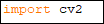
\includegraphics[width=0.3\linewidth]{images/1.PNG}
    \caption{Memasukan library openCV}
\end{figure}
\\- Proses face detection, untuk melakukan proses deteksi wajah akan menggunakan algoritma \emph{haarcascade}. Dengan fungsi \textbf{cv2.CascadeClassifier}
\begin{figure}[h!]
    \centering
    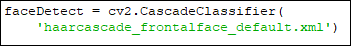
\includegraphics[width=0.7\linewidth]{images/2.PNG}
    \caption{Memasukan library openCV}
\end{figure}
\\- Memasukan video, \textbf{cv2.VideoCapture} merupakan fungsi untuk membaca video yang akan dijadikan \emph{sample} dan bisa juga untuk menampilkan frame kamera yang terkoneksi dengan komputer.
\begin{figure}[h!]
    \centering
    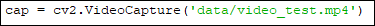
\includegraphics[width=0.7\linewidth]{images/3.PNG}
    \caption{Memasukan video}
\end{figure}
\\- Membuka video/kamera dan merubah warna. Kode pada baris pertama digunakan untuk membuka video atau kamera yang terhubung, baris kedua merupakan
kode untuk mengubah warna citra menjadi hitam putih menggunakan \textbf{cv2.cvtColor}
\begin{figure}[h!]
    \centering
    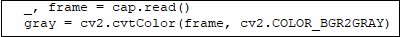
\includegraphics[width=0.7\linewidth]{images/4.PNG}
    \caption{Membuka video dan ubah warna cira}
\end{figure}
\\- Fungsi untuk mendeteksi wajah, menggunakan fungsi \textbf{detectMultiScale}
\begin{figure}[h!]
    \centering
    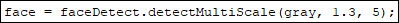
\includegraphics[width=0.7\linewidth]{images/5.PNG}
    \caption{Deteksi wajah}
\end{figure}
\\- Fungsi untuk membuat bingkai tanda jika wajah terdeteksi oleh sistem menggunakan \textbf{cv2.rectangle} jika berbentuk persegi. Dan fungsi \textbf{cv2.imshow} untuk menjalankan sistem yang telah dibuat.
\begin{figure}[h!]
    \centering
    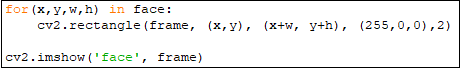
\includegraphics[width=0.75\linewidth]{images/6.PNG}
    \caption{Kode bingkai wajah}
\end{figure}
\\Berikut adalah seluruh kode dan hasil untuk sistem deteksi wajah:
\begin{figure}[h!]
    \centering
    \includegraphics[width=0.75\linewidth]{images/full.PNG}
    \caption{Kode deteksi wajah}
\end{figure}
\begin{figure}[h!]
    \centering
    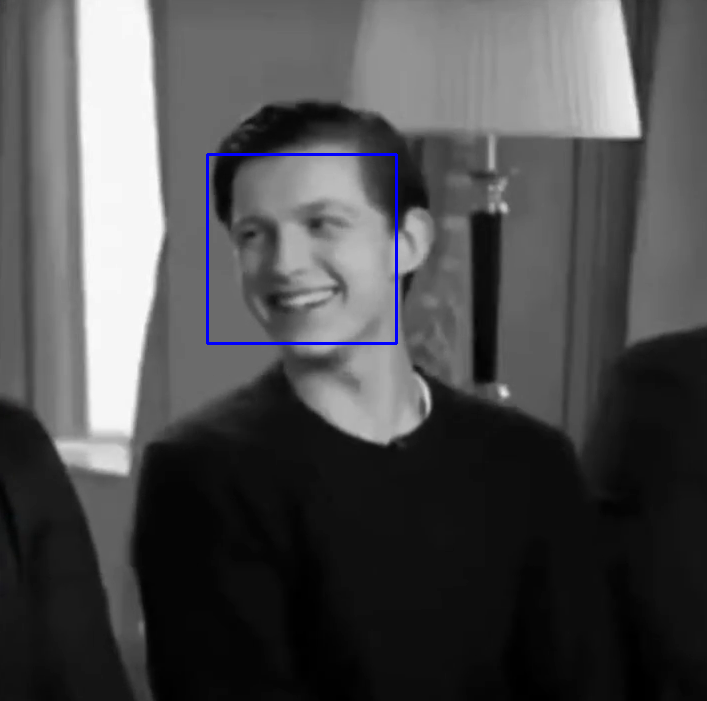
\includegraphics[width=0.33\linewidth]{images/HASIL 1.PNG}
    \includegraphics[width=0.34\linewidth]{images/HASIL 2.PNG}
    \caption{Hasil deteksi wajah}
\end{figure}